
% 脚の可動班を表示するプログラムの説明

\chapter{脚の可動域を表示するプログラム}\label{chapter:leg_range_python}

\section{概要}
近似的な脚の可動域が適切であるかを評価するためには,
PhantomXの可動域を正確に把握する必要がある.
そのためには可動域の可視化を行うことが必要だろう.
そこで,PhantomXの脚の可動域を可視化するプログラムを作成した.
プログラムは簡単のためPythonを用いて作成しており,
GitHubを通じてだれでも利用できるようにしている.
以下にプログラムの導入方法を説明し,
プログラムの仕様について述べる.

\section{導入方法}
プログラムはGitHubを通じて公開しているため,
まずはGitHubからプログラムをダウンロードする方法を説明する.
そしてPythonのプログラムをコンパイルする方法を説明する.

\subsection{Gitの使用方法}
Gitとは,ソースコードなどの変更履歴を記録・追跡するための分散型バージョン管理システムである.
かみ砕いて言うならば,Googleドキュメントの履歴機能や,
Microsoft Wordの変更履歴機能のようなシステムをさまざまなプログラムのソースコードに対して適用したものといえるだろう.
また,GitHubとは,Gitを用いてソースコードを管理するためのサービスである.
GitHubを用いることで,ソースコードの変更履歴を保存することができるだけでなく,
自分のソースコードを公開したり,他の人が作成したソースコードをダウンロードしたりすることもできる.

\subsubsection{Gitのインストール}
Gitを使うため,まずはGitをインストールする必要がある.
次のリンクからGitのインストーラをダウンロードし,実行する.
インストーラではオプションの設定を変更する必要はないため,
すべてのページで変更をせずに「Next」を選択してインストールを行う.

\begin{itemize}
  \item Git for Windows https://git-scm.com/downloads (アクセス日 2023/12/30)
\end{itemize}

Gitは多くのアプリケーションとは違い,コマンドを用いて操作を行う.
そのため,インストールが完了しても,Gitのアプリケーションが起動することはない.
Gitのインストールが成功したかどうかは,コマンドを用いて確認する.
インストールが完了した場合,Gitのコマンドが使用できるようになっているはずである.
1度パソコンを再起動したのち,\figref{fig:app_b_git_bash}のように
スタートメニューに「Git Bash」と入力してGit Bashを起動する.
Git Bashが起動したら,\coderef{lst:app_b_git_version}のコマンドを入力する.
\figref{fig:app_b_git_version}のようにGitのバージョンが表示されれば,インストールは成功している.
\\
\begin{lstlisting}[caption=Gitのバージョン確認コマンド, label=lst:git_version]
  git --version
\end{lstlisting}

\begin{figure}[h]
  \begin{tabular}{cc}
      \begin{minipage}{.45\textwidth}
          \centering
          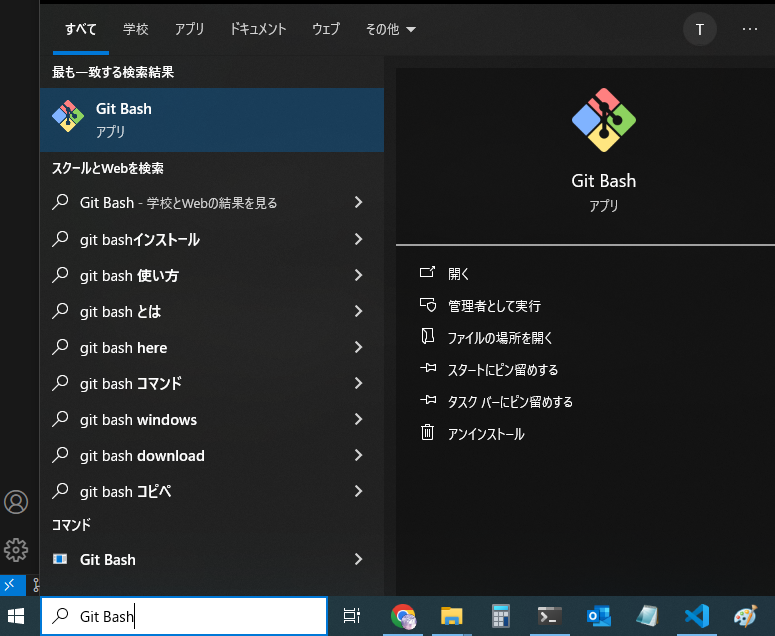
\includegraphics[width=1.0\linewidth]{figure/appendix/git_bash.png}
          \caption{Git Bash}
          \label{fig:app_b_git_bash} % chktex 24
      \end{minipage}
      \begin{minipage}{.45\textwidth}
          \centering
          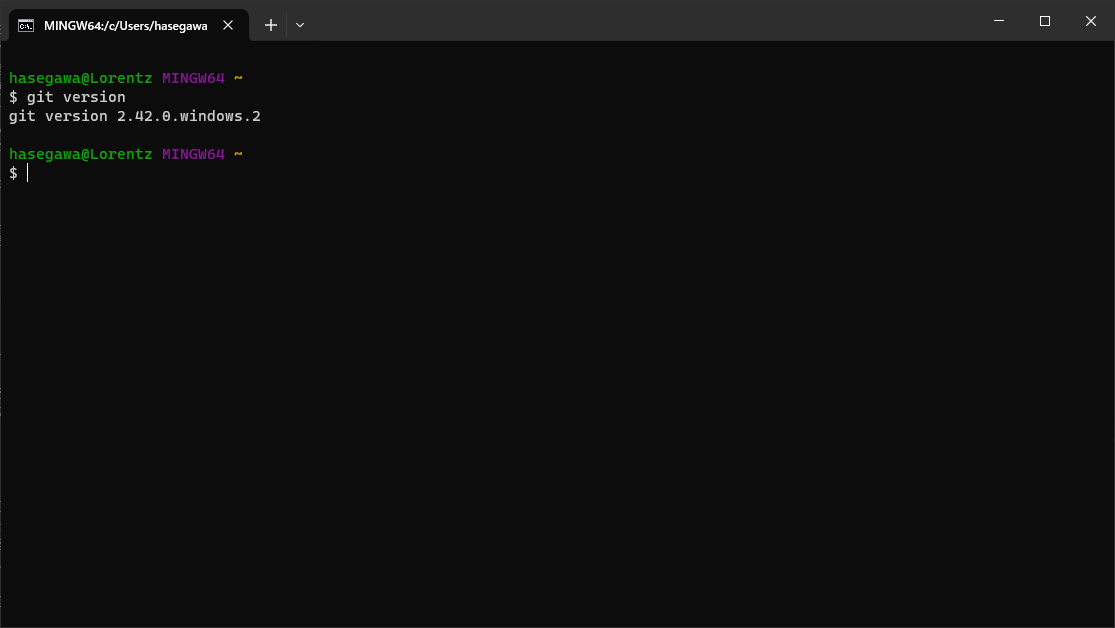
\includegraphics[width=1.0\linewidth]{figure/appendix/git_version.png}
          \caption{Display Git Version}
          \label{fig:app_b_git_version} % chktex 24
      \end{minipage}
  \end{tabular}
\end{figure}

\subsubsection{GitHubのアカウント作成}
次にGitHubからプログラムをダウンロードする方法を説明する.
まずはGitHubのアカウントを作成する.
GitHubのアカウントを作成するためには,次のリンクからアクセスし,
アカウント作成の手順にしたがってアカウントを作成する.
アカウントが作成できれば,次のような画面が表示される.

\begin{itemize}
  \item GitHub https://github.com/ (アクセス日 2024/02/17)
  \item GitHubでのアカウントの作成 https://docs.github.com/ja/get-started/start-your-journey/creating-an-account-on-github (アクセス日 2024/02/17)
\end{itemize}

\subsubsection{レポジトリのフォーク,クローン}
GitHubからプログラムのダウンロードを行うための手順を説明する.
しかし,Gitの操作においては日常的に聞きなれないであろう用語が多く出てくるため,
まずはそれらの用語を説明する.
\begin{itemize}
  \item レポジトリ(repository):ファイルやディレクトリの変更履歴を記録する場所.PCでいうところのフォルダ.
  \item フォーク(fork):他のユーザのレポジトリを自分のアカウントにコピーすること
  \item クローン(clone):GitHub上のレポジトリを自分のパソコンにダウンロードすること
\end{itemize}

さて,プログラムをダウンロードするためには,まずはGitHub上のレポジトリを自分のアカウントにフォークする必要がある.
以下に脚の可動範囲を表示するプログラムのレポジトリのURLを示す.

\begin{itemize}
  \item 脚の可動範囲を表示するプログラム \url{https://github.com/hase111111/phantomx_leg_display/tree/main} (アクセス日 2024/02/17)
\end{itemize}

\subsection{pythonのコンパイル方法}
本項目では,Windows 10におけるpythonのコンパイル方法を説明する.
当方の開発環境はWindows 10であるため,Windows 10におけるpythonのコンパイル方法についてのみ説明するものとし,
Mac OSやLinuxにおけるpythonのコンパイル方法については,ここでは説明しない.
(しかし,「python Mac 環境構築」,「python Linux 環境構築」などで検索すると最適な方法が見つかるだろう.
とくにLinuxにおいては環境構築は非常に簡単である.)

Windows 10におけるpythonの使用方法として,pipを用いた環境を使用する方法があるが,
ここではAnacondaを用いた環境を使用する方法を説明する.
Anacondaはpythonのパッケージ管理システムであり,pythonの環境構築を簡単に行うことができる.
注意点としてcondaとpipは別のパッケージ管理システムであるため,
Anacondaを使用する場合はpipコマンドを使用してはならない.

\section{プログラムの仕様}

